\chapter{O editor HTML}

\index{editor HTML}

\section{Introdução}

Em quase todas as Atividades e Recursos em Moodle é necessário usar um editor de textos para inserir informações. O editor, que guarda boa semelhança com um editor de textos comuns é, na verdade, uma interface gráfica para a construção de textos na linguagem HTML (Hyper Text Markup Language), usada para a construção de páginas na Internet.

Neste apêndice são descritas as principais características desse editor.

\section{A barra de ferramentas}

\index{editor!ferramentas}

A Figura A.1 mostra a barra de ferramentas do editor.

\begin{figure}
 \begin{center}
 \fbox{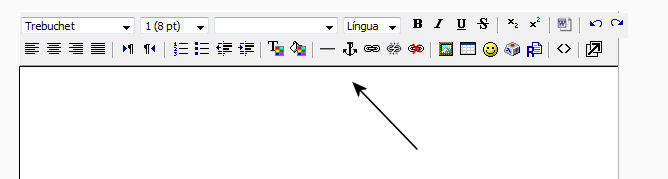
\includegraphics[width=0.6\textwidth]{imagem/cap0/fig-a-01.jpg}}
  \caption{Barra de ferramentas do editor de textos}
 \end{center}
\end{figure}

\section{Alterações no texto}

\index{editor!alterando texto}

Para promover alterações no texto podem ser usadas as ferramentas destacadas na Figura A.2.

\begin{figure}
 \begin{center}
 \fbox{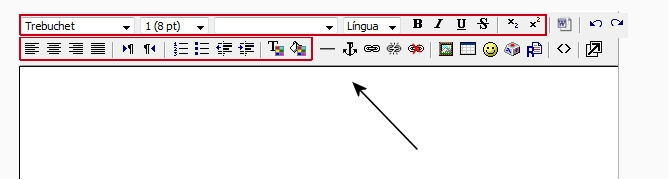
\includegraphics[width=0.6\textwidth]{imagem/cap0/fig-a-01_t.jpg}}
  \caption{Alterações no texto}
 \end{center}
\end{figure}

O texto a ser alterado deve ser selecionado com o botão esquerdo do mouse. Depois, escolhe-se a alteração desejada seguindo as indicações da Tabela A.1.

Quando se aciona (
\includegraphics[width=0.3cm]{imagem/cap0/ed_color_fg.jpg}) e 
(
\includegraphics[width=0.3cm]{imagem/cap0/ed_color_bg.jpg}) tem-se acesso à paleta de cores mostrada na Figura A.3.

\begin{figure}{l}
 \begin{center}
 \fbox{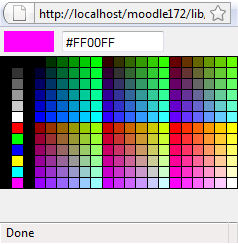
\includegraphics[width=0.3\textwidth]{imagem/cap0/fig-a-02.jpg}}
  \caption{Paleta de cores}
 \end{center}
\end{figure}

A linha horizontal (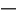
\includegraphics[width=0.4cm]{imagem/cap0/hr.jpg}) pode ser muito útil para agrupar e organizar informações na tela de abertura de um curso.

\begin{table}
\begin{center}
 \begin{tabular}{m{0.5cm} m{6.0cm}} \\
  
\includegraphics[width=0.4cm]{imagem/cap0/bold.jpg} & \textbf{Negrito} \\
  
\includegraphics[width=0.4cm]{imagem/cap0/italic.jpg} & \textit{Itálico} \\
  
\includegraphics[width=0.4cm]{imagem/cap0/underline.jpg} & \underline{Sublinhado} \\
  
\includegraphics[width=0.4cm]{imagem/cap0/strike.jpg} & \sout{Riscado} \\
  
\includegraphics[width=0.4cm]{imagem/cap0/sub.jpg} & $._{Subscrito}$ \\
  
\includegraphics[width=0.4cm]{imagem/cap0/sup.jpg} & $.^{Superescrito}$ \\ 
  
\includegraphics[width=0.4cm]{imagem/cap0/align_left.jpg} & Alinhar texto à esquerda \\
  
\includegraphics[width=0.4cm]{imagem/cap0/align_center.jpg} & Centralizar o texto \\
  
\includegraphics[width=0.4cm]{imagem/cap0/align_right.jpg} & Alinhar texto à direita \\ 
  
\includegraphics[width=0.4cm]{imagem/cap0/align_justify.jpg} & Justificar o texto \\
  
\includegraphics[width=0.4cm]{imagem/cap0/left_to_right.jpg} & Escrever da esquerda para a direita \\
  
\includegraphics[width=0.4cm]{imagem/cap0/right_to_left.jpg} & Escrever da direita para a esquerda \\
  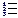
\includegraphics[width=0.4cm]{imagem/cap0/list_num.jpg} & Listas numeradas \\
  
\includegraphics[width=0.4cm]{imagem/cap0/list_bullet.jpg} & Listas com marcadores \\
  
\includegraphics[width=0.4cm]{imagem/cap0/indent_less.jpg} & Reduzir distância da margem (identação) \\
  
\includegraphics[width=0.4cm]{imagem/cap0/indent_more.jpg} & Aumentar distância da margem (identação) \\
  
\includegraphics[width=0.4cm]{imagem/cap0/ed_color_fg.jpg} & Alterar cor do texto \\
  
\includegraphics[width=0.4cm]{imagem/cap0/ed_color_bg.jpg} & Alterar cor do fundo \\
  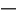
\includegraphics[width=0.4cm]{imagem/cap0/hr.jpg} & Inserir uma linha horizontal \\ \hline
 \end{tabular}
\caption{Ferramentas de alteração de textos}
\end{center}
\end{table}

\section{Links e âncoras}

\index{link}
\index{âncora}

A Figura A.4 mostra as ferramentas para trabalhar com links e âncoras.

\begin{figure}
 \begin{center}
 \fbox{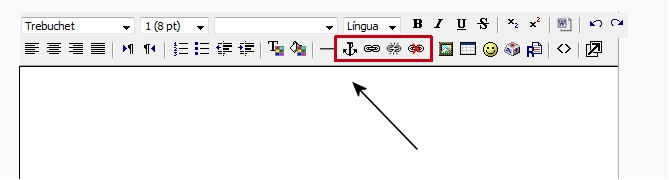
\includegraphics[width=0.6\textwidth]{imagem/cap0/fig-a-04.jpg}}
  \caption{Trabalhando com links e âncoras}
 \end{center}
\end{figure}

A função de cada ferramenta é descrita na Tabela A.2.

\begin{table}
\begin{center}
 \begin{tabular}{m{0.5cm} m{4.0cm}} \\
  
\includegraphics[width=0.4cm]{imagem/cap0/anchor.jpg} & \ Criar uma âncora \\
  
\includegraphics[width=0.4cm]{imagem/cap0/link.jpg} & Inserir um link web \\
  
\includegraphics[width=0.4cm]{imagem/cap0/unlink.jpg} & Remover um link \\
  
\includegraphics[width=0.4cm]{imagem/cap0/nolink.jpg} & Evitar links automáticos \\  \hline
 \end{tabular}
\caption{Ferramentas para links e âncoras}
\end{center}
\end{table}

\subsection{Inserir links}

Ao clicar na ferramenta 
\includegraphics[width=0.4cm]{imagem/cap0/link.jpg} aparece a tela mostrada na Figura A.5. O exemplo mostrado na figura permite associar à palavra Moodle o endereço internet oficial do Moodle (www.moodle.org). Clicando na palavra Moodle abre-se uma nova tela no navegador internet com o site oficial.

\begin{figure}
 \begin{center}
 \fbox{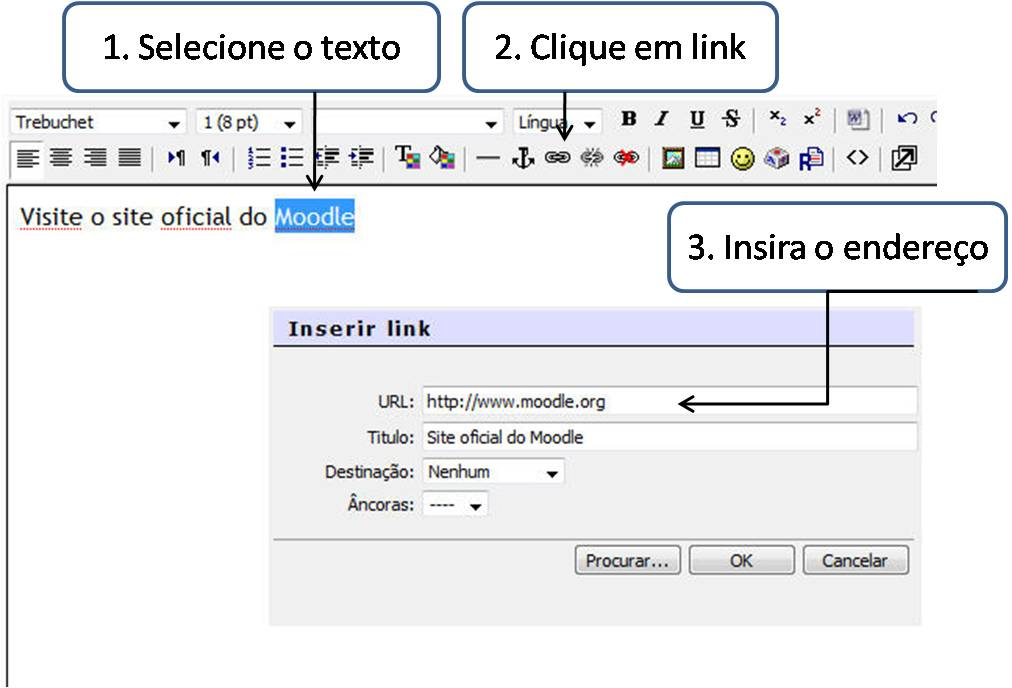
\includegraphics[width=0.6\textwidth]{imagem/cap0/fig-a-05.jpg}}
  \caption{Criando um link}
 \end{center}
\end{figure}

\subsection{Remover link}

\index{link!remover}

Quando uma palavra (ou frase) é linkada a um endereço web é possível remover esse link selecionando a palavra e clicando no ícone 
\includegraphics[width=0.4cm]{imagem/cap0/unlink.jpg}.

\subsection{Âncoras}

\index{âncora}

Uma âncora html (
\includegraphics[width=0.4cm]{imagem/cap0/ed_anchor.jpg}) permite linkar palavras (ou textos) a outras palavras (ou textos) dentro de uma mesma tela.

Uma possível utilização de âncoras é a necessidade de se trabalhar com um texto relativamente longo (duas ou mais telas de computador) sem usar o recurso Livro. Se o texto é longo, e inevitável, é possível criar um índice usando âncoras. Veja-se o exemplo mostrado na Figura A.6.

\begin{figure}
 \begin{center}
 \fbox{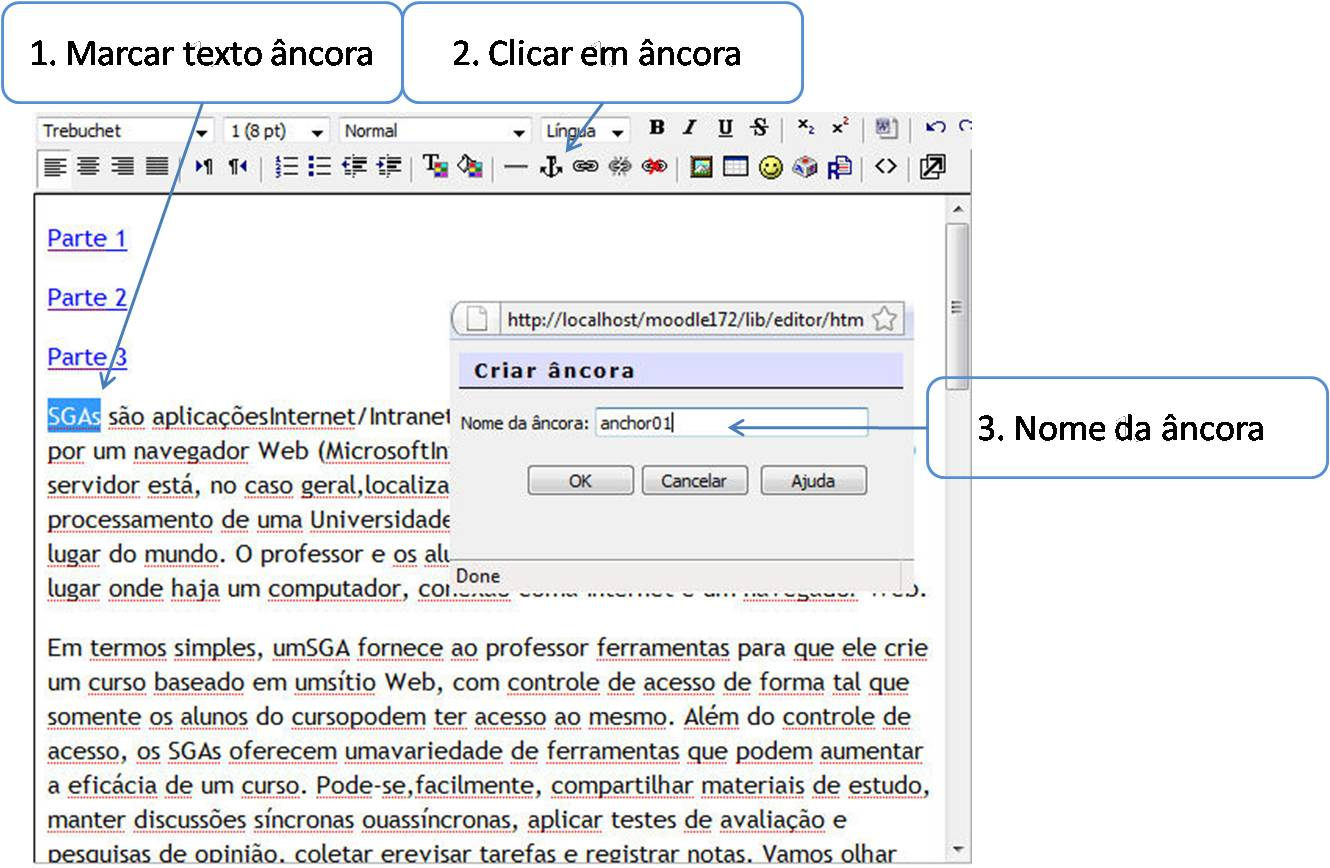
\includegraphics[width=0.6\textwidth]{imagem/cap0/fig-a-06.jpg}}
  \caption{Trabalhando com âncoras}
 \end{center}
\end{figure}

Observe-se, na figura, as palavras Parte 1, Parte 2 e Parte 3, em azul. Essas palavras são links para palavras que pertencem ao texto mostrado. As palavras são linkadas, neste caso, não para endereços Internet mas para outras palavras no próprio texto. Essas outras palavras são marcadas como âncoras.

Os passos a serem dados são detalhados a seguir.

\begin{itemize}
 \item Escolher as palavras que serão âncoras. Aquelas para as quais o índice deve conduzir o leitor.
 \item Marcar cada uma delas, clicar no ícone 
\includegraphics[width=0.4cm]{imagem/cap0/anchor.jpg} e escolher um nome para a âncora (por exemplo, anchor01, anchor02, etc.).
 \item Marcar cada uma das palavras das quais se pretende conduzir o leitor para as palavras âncora. Para cada uma delas, clicar em 
\includegraphics[width=0.4cm]{imagem/cap0/link.jpg} e, em lugar de indicar um link na internet, escolher a correspondente âncora. Veja-se Figura A.7.
\end{itemize}

\begin{figure}
 \begin{center}
 \fbox{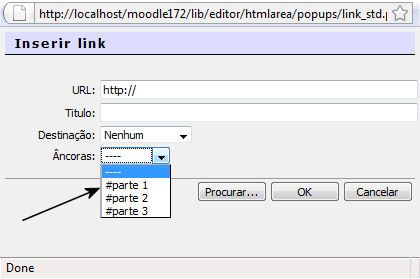
\includegraphics[width=0.5\textwidth]{imagem/cap0/fig-a-07.jpg}}
  \caption{Fazendo um link para uma âncora}
 \end{center}
\end{figure}

\index{link!para âncora}

\section{Figuras, emoticons e caracteres especiais}

\index{editor!figuras}
\index{editor!emoticons}
\index{editor!caracteres}

A Figura A.8 mostra os links para a inserção de figuras, emoticons e caracteres especiais.

\begin{figure}
 \begin{center}
 \fbox{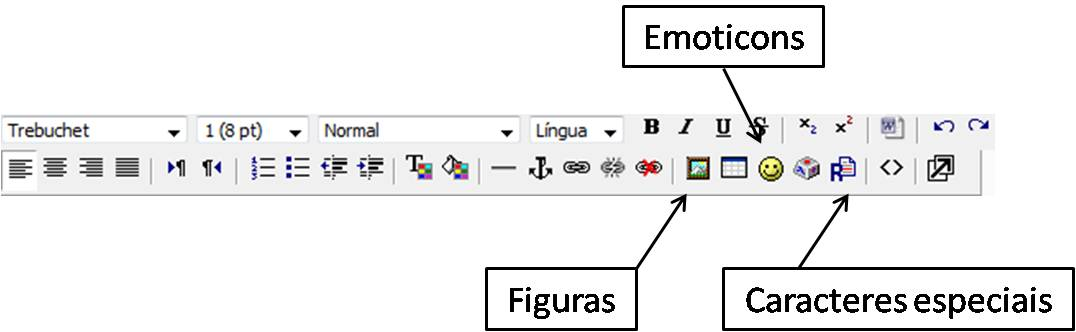
\includegraphics[width=0.6\textwidth]{imagem/cap0/fig-a-08.jpg}}
  \caption{Figuras, emoticons e caracteres especiais}
 \end{center}
\end{figure}

\subsection{Figuras}

Para inserir figuras em um texto qualquer usando o editor HTML clica-se no ícone 

\includegraphics[width=0.4cm]{imagem/cap0/image.jpg}, na barra de ferramentas do editor. A tela de inserção é mostrada na Figura A.9.

\begin{figure}
 \begin{center}
 \fbox{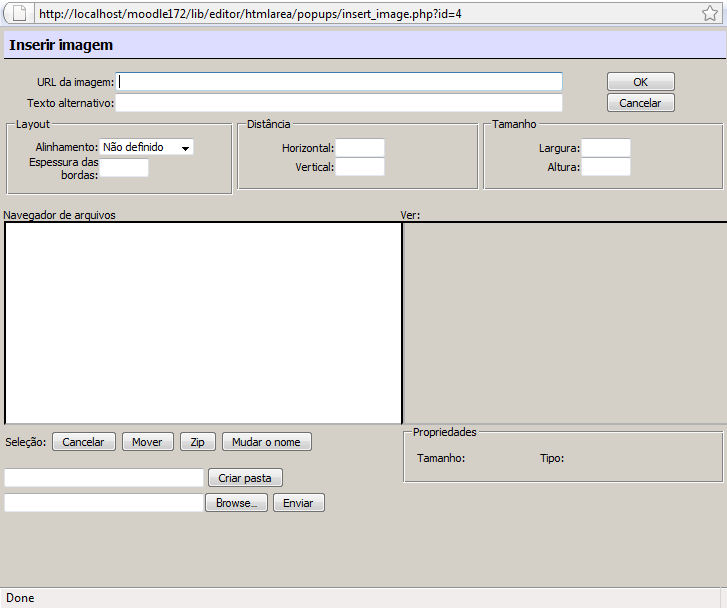
\includegraphics[width=0.6\textwidth]{imagem/cap0/fig-a-09.jpg}}
  \caption{Inserindo uma figura}
 \end{center}
\end{figure}

Observa-se, na Figura A.9, que o campo Navegador de arquivos está sem conteúdo. Isto significa que nenhuma figura foi ainda enviada para a seção Arquivos, no bloco Administração do curso. As figuras a serem inseridas em um texto no ambiente devem, antes ser enviadas do computador do professor para a seção Arquivos do curso. Isto pode ser feito ou clicando-se em Browse... (Navegar a depender do computador) para procurar o arquivo com a figura. Um exemplo é mostrado na Figura A.10. Pretende-se enviar ao ambiente a figura que está no arquivo fig02-01. Clicando em Open (Abrir) e depois em Enviar na tela da Figura A.9, o resultado é mostrado na Figura A.11.

\index{figura!enviar}

\begin{figure}
 \begin{center}
 \fbox{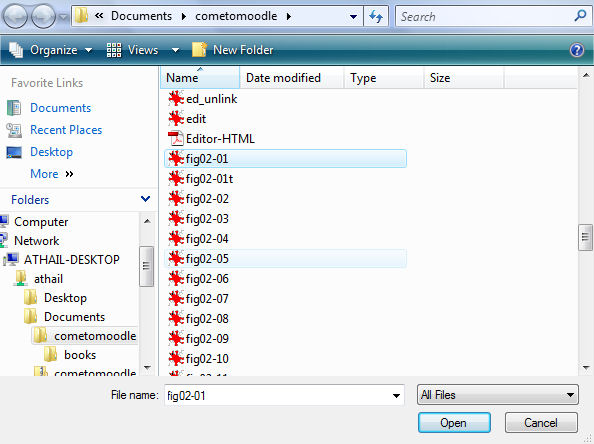
\includegraphics[width=0.6\textwidth]{imagem/cap0/fig-a-10.jpg}}
  \caption{Enviando uma figura para o ambiente}
 \end{center}
\end{figure}

\begin{figure}
 \begin{center}
 \fbox{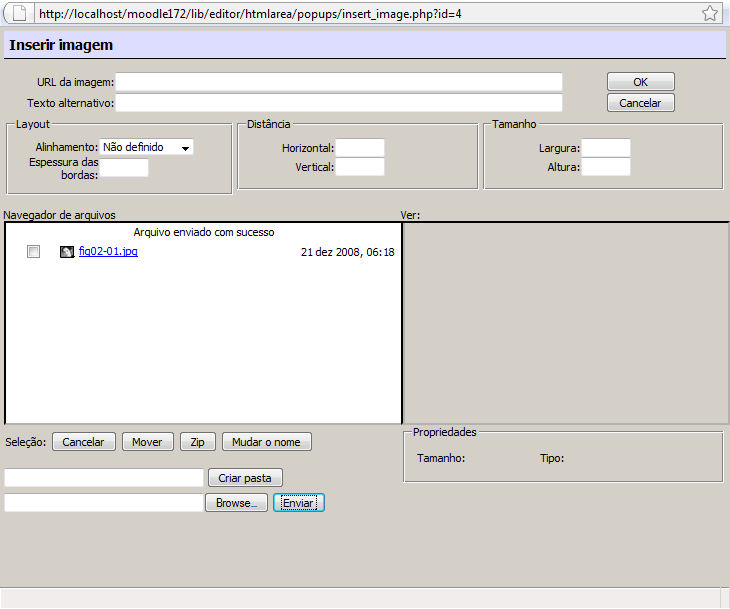
\includegraphics[width=0.6\textwidth]{imagem/cap0/fig-a-11.jpg}}
  \caption{Figura enviada para o ambiente}
 \end{center}
\end{figure}

Agora a imagem enviada pode ser selecionada e inserida no texto em construção. Um resumo dos procedimentos é mostrado na Figura A.12.

\begin{figure}
 \begin{center}
 \fbox{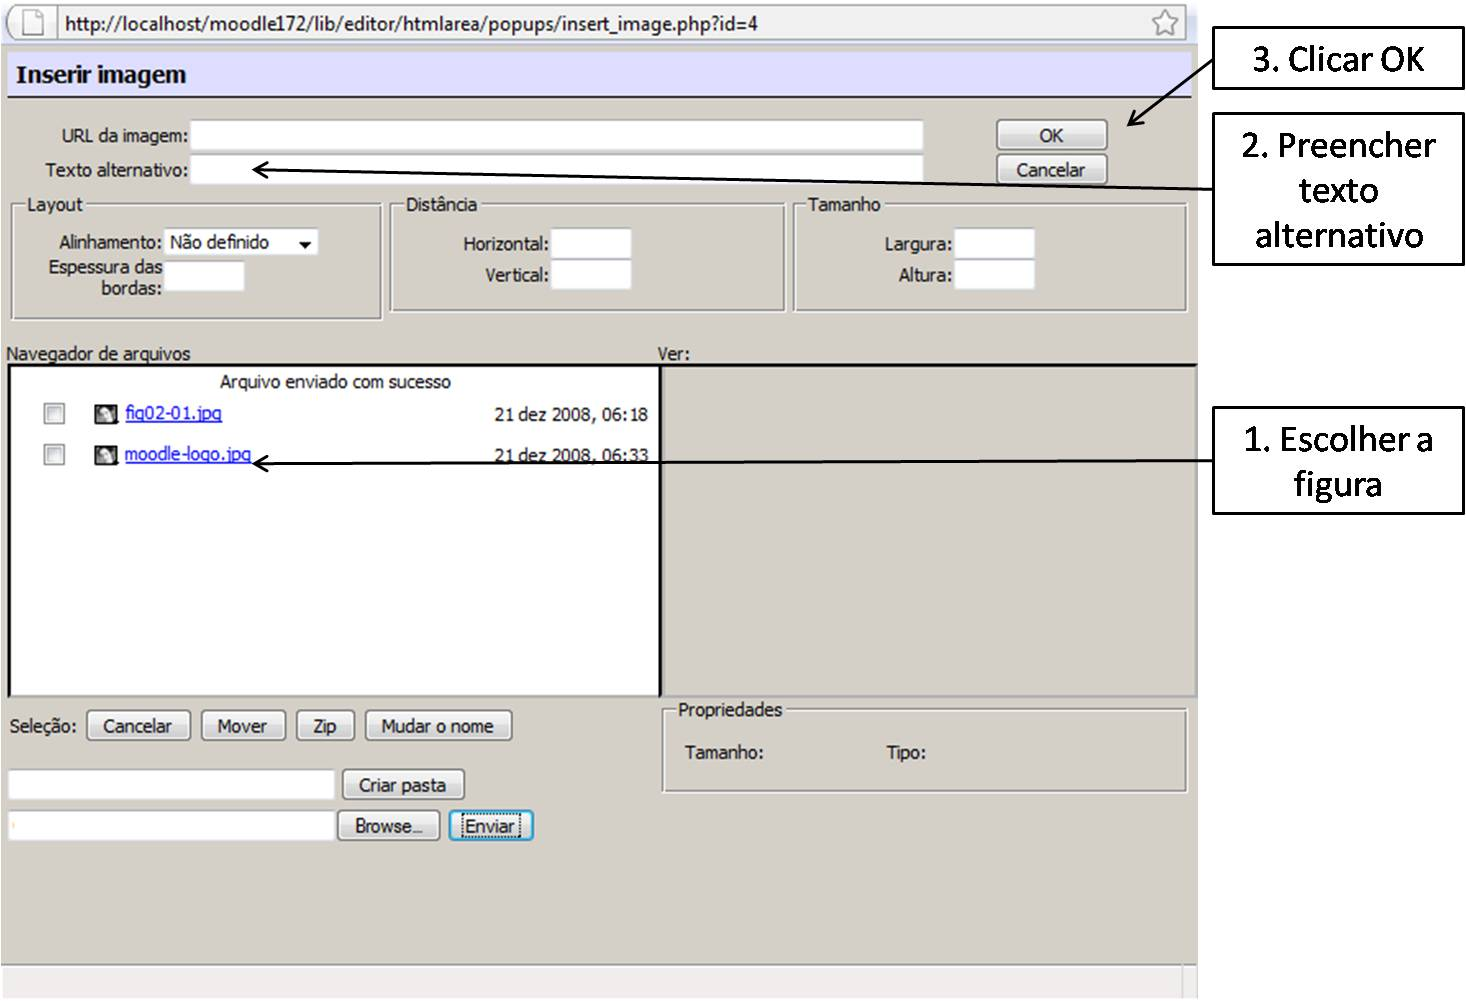
\includegraphics[width=0.6\textwidth]{imagem/cap0/fig-a-12.jpg}}
  \caption{Inserindo figura - roteiro final}
 \end{center}
\end{figure}

\subsection{Emoticons}

\index{emoticons}

Clicando em 
\includegraphics[width=0.4cm]{imagem/cap0/emoticons.jpg} tem-se acesso à tela mostrada na Figura A.13.

\begin{figure}
 \begin{center}
 \fbox{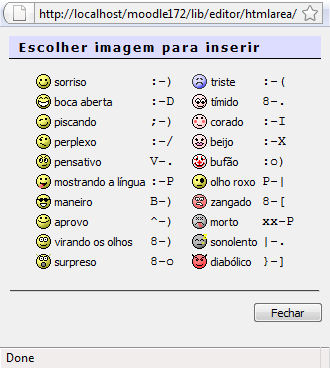
\includegraphics[width=0.6\textwidth]{imagem/cap0/fig-a-13.jpg}}
  \caption{Emoticons}
 \end{center}
\end{figure}

Clicando em qualquer dos emoticons (ou usando o código html mostrado na frente de imagem) a imagem é inserida no texto na posição onde está o cursor.

\subsection{Caracteres especiais}

\index{caracteres especiais}

Clicando no ícone 
\includegraphics[width=0.4cm]{imagem/cap0/char.jpg} tem-se acesso à tela mostrada na Figura A.14. Basta escolher o caracter e ele será inserido no texto, na posição em que está o cursor.

\begin{figure}
 \begin{center}
 \fbox{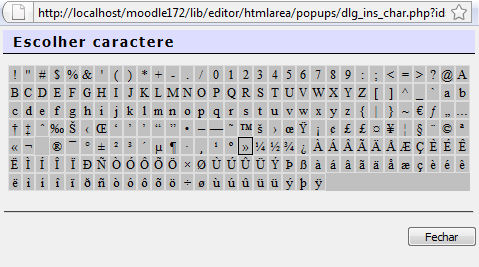
\includegraphics[width=0.6\textwidth]{imagem/cap0/fig-a-14.jpg}}
  \caption{Caracteres especiais}
 \end{center}
\end{figure}

\section{Tabelas}

\index{tabelas}
\index{editor!tabelas}

Clicando no ícone 
\includegraphics[width=0.4cm]{imagem/cap0/insert_table.jpg} tem-se acesso à tela mostrada na Figura A.15.

\begin{figure}
 \begin{center}
 \fbox{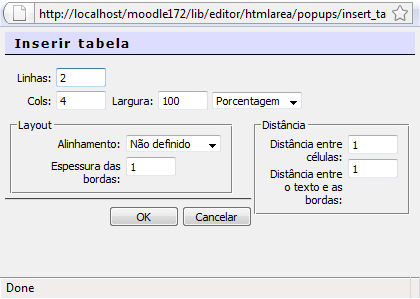
\includegraphics[width=0.6\textwidth]{imagem/cap0/fig-a-15.jpg}}
  \caption{Inserindo uma tabela}
 \end{center}
\end{figure}

\index{pixels}

Em Linhas e Cols define-se o número de linhas e colunas que a tabela deve ter. A largura da tabela pode ser estabelecida em porcentagem da largura da tela ou em pixels. \footnote{http://pt.wikipedia.org/wiki/Pixel}

A configuração do alinhamento da tabela (esquerdo, direito, topo do texto, centro, etc.) e a espessura das bordas são definidos na área Layout.

Para auxiliar na configuração de tabelas deve-se clicar no ícone \includegraphics[width=0.4cm]{imagem/cap0/fullscreen.jpg} e observar que aparece uma terceira linha de ferramentas na barra do editor. Veja-se Figura A.16.

\begin{figure}
 \begin{center}
 \fbox{\includegraphics[width=0.6\textwidth]{imagem/cap0/fig-a-16.jpg}}
  \caption{Ferramentas para edição de tabelas}
 \end{center}
\end{figure}

A Tabela A.3 mostra a função de cada uma das novas ferramentas.

\begin{table}
\begin{center}
 \begin{tabular}{m{0.5cm} m{6.0cm}} \\
  \includegraphics[width=0.4cm]{imagem/cap0/table-prop.jpg} & \ Configurar propriedades da tabela \\
  \includegraphics[width=0.4cm]{imagem/cap0/row-prop.jpg} & Configurar linhas da tabela \\
  \includegraphics[width=0.4cm]{imagem/cap0/row-insert-above.jpg} & Inserir linha acima \\
  \includegraphics[width=0.4cm]{imagem/cap0/row-insert-under.jpg} & Inserir linha abaixo \\
  \includegraphics[width=0.4cm]{imagem/cap0/row-delete.jpg} & Excluir linha \\
  \includegraphics[width=0.4cm]{imagem/cap0/row-split.jpg} & Dividir linha \\
  \includegraphics[width=0.4cm]{imagem/cap0/col-insert-before.jpg} & Inserir coluna à esquerda \\
  \includegraphics[width=0.4cm]{imagem/cap0/col-insert-after.jpg} & Inserir coluna à direita \\
  \includegraphics[width=0.4cm]{imagem/cap0/col-delete.jpg} & Excluir coluna \\
  \includegraphics[width=0.4cm]{imagem/cap0/col-split.jpg} & Dividir coluna \\
  \includegraphics[width=0.4cm]{imagem/cap0/cell-prop.jpg} & Propriedades de uma célula \\
  \includegraphics[width=0.4cm]{imagem/cap0/cell-insert-before.jpg} & Inserir célula antes da atual \\
  \includegraphics[width=0.4cm]{imagem/cap0/cell-insert-after.jpg} & Inserir célula depois da atual \\
  \includegraphics[width=0.4cm]{imagem/cap0/cell-delete.jpg} & Remover célula atual \\
  \includegraphics[width=0.4cm]{imagem/cap0/cell-merge.jpg} & Juntar células selecionadas \\
  \includegraphics[width=0.4cm]{imagem/cap0/cell-split.jpg} & Dividir células \\ \hline
 \end{tabular}
\caption{Ferramentas para edição de tabelas}
\end{center}
\end{table}

\begin{quotation}
 Cabe aqui uma observação importante. O editor html usado em Moodle é, na verdade, uma interface gráfica para faciligar a edição de textos na linguagem html, usada para construir páginas na Internet. O uso de tabelas para organizar texto e informações em uma página html é muito útil. Assim, o domínio da construção de tabelas deve ser um objetivo do leitor. Experimentando, treinando, refazendo e, talvez, lendo um pouco sobre html tem-se grande ganho na clareza e organização dos textos criados.
\end{quotation}

\section{Outras ferramentas}

A Tabela A.4 mostra outras ferramentas de edição. O leitor é incentivado a experimentar cada uma delas. Tudo pode ser desfeito ou feito novamente. Em especial, chama-se a atenção para \includegraphics[width=0.4cm]{imagem/cap0/ed_html.jpg}. É interessante aprender um pouco sobre a linguagem html observando o texto como visto pelo leitor e sua real construção na linguagem html. É também uma forma de aprender a linguagem.

\begin{table}
\begin{center}
 \begin{tabular}{m{0.5cm} m{6.0cm}} \\
  \includegraphics[width=0.4cm]{imagem/cap0/ed_replace.jpg} & \ Procurar e substituir texto \\
  \includegraphics[width=0.4cm]{imagem/cap0/fullscreen_maximize.jpg} & Expandir a tela do editor \\
  \includegraphics[width=0.4cm]{imagem/cap0/fullscreen_minimize.jpg} & Reduzir a tela do editor \\
  \includegraphics[width=0.4cm]{imagem/cap0/ed_wordclean.jpg} & Limpar textos produzidos em Word \\
  \includegraphics[width=0.4cm]{imagem/cap0/ed_undo.jpg} & Desfazer a última ação \\
  \includegraphics[width=0.4cm]{imagem/cap0/ed_redo.jpg} & Repetir a última ação \\
  \includegraphics[width=0.4cm]{imagem/cap0/ed_html.jpg} & Mostrar o texto na linguagem html \\ \hline
 \end{tabular}
\caption{Outras ferramentas do editor}
\end{center}
\end{table}

